\section{Аналитический раздел}

В данном разделе проводится анализ предметной области оценки кредитоспособности физических лиц в банковских системах. Описываются основные понятия, используемые в кредитном скоринге, а также рассматриваются современные методы машинного обучения, применяемые для оценки кредитного риска, включая алгоритм градиентного бустинга деревьев решений. Выполняется обзор существующих решений в области кредитного скоринга и приводится сравнительный анализ традиционных статистических методов и алгоритмов машинного обучения. На основании проведенного анализа формулируется цель работы и осуществляется формализация постановки задачи в виде IDEF0-диаграммы.

\subsection{Анализ предметной области}

Кредитный риск представляет собой вероятность того, что заемщик или контрагент банка не выполнит свои обязательства в соответствии с согласованными условиями. Для банков кредитный риск является одним из ключевых видов риска, поскольку его реализация может привести к финансовым потерям и ухудшению качества кредитного портфеля. Управление кредитным риском предполагает не только оценку отдельных заемщиков, но и контроль совокупного уровня риска по кредитному портфелю \cite{BaselCreditRisk}.

Кредитный риск включает несколько аспектов, таких как дефолт заемщика (невозврат кредита), просрочка платежей или недобросовестное поведение заемщика. Оценка и управление кредитным риском являются критическими задачами для банков, поскольку неправильное принятие решений может привести к финансовым потерям и негативным последствиям для банковской организации. Кредитор оценивает кредитоспособность, анализируя информацию, предоставленную заемщиком для получения кредита \cite{Konovalova}. Оценка кредитного риска является одним из основных инструментов, которые используются финансовыми организациями при выдаче кредитов. Скоринговые методы в банковских системах являются важной частью процесса кредитования и управления рисками.

Скоринг стал использоваться не только при оценке кредитных рисков, но и в маркетинге для определения вероятности покупки тех или иных продуктов теми или иными покупателями. При работе с должниками, если клиент задерживается с очередным платежом, скоринг позволяет выявить, какой способ воздействия будет наиболее эффективным. Также эти методы используются для выявления мошенничества с кредитными картами и для оценки вероятности перехода клиента к конкуренту и в других подобных ситуациях \cite{Zaernuk}.

Кредитный скоринг представляет собой статистический метод оценки вероятности того, что заявитель на кредит, действующий заемщик или контрагент допустит дефолт либо просрочку платежа. В рамках скорингового подхода сведения о заемщике преобразуются в числовую оценку, которая используется для ранжирования клиентов по уровню кредитного риска и поддержки решения о предоставлении кредита. Таким образом, скоринговая модель позволяет формализовать процесс оценки кредитоспособности и сделать процедуру принятия кредитного решения более объективной \cite{WorldBankCreditScoring}.

Наиболее используемые кредитные скоринговые системы:
\begin{itemize}
  \item скоринг заявлений (англ. Application scoring);
  \item поведенческий скоринг (англ. Behavioral scoring);
  \item коллекторский скоринг (англ. Collection scoring);
  \item противомошеннический скоринг (англ. Fraud scoring).
\end{itemize}

Скоринг заявлений -- это определение кредитоспособности (уровня риска дефолта) заявителя при принятии решения о предоставлении кредита на основании данных, доступных в момент подачи заявления. Фактически это анализ анкетных данных заемщика и вычисление рисков невозврата кредита. При этом принимается не только решение о предоставлении кредита, но и о размере и условиях кредитования. Основная цель при внедрении -- экспресс-оценка заемщика и сокращение времени на изучение документов \cite{Tkachev}.

Коллекторский скоринг -- это решение ключевых задач коллекторской деятельности, а именно планирование и осуществление своевременных и целенаправленных действий по управлению взаимоотношениями с должниками начиная с момента первого возникновения просрочки. Эффективный процесс своевременного предупреждения просрочек является очень важным для снижения затрат по работе с долгами и залоговым имуществом. Внедрение в банке системы коллекторского скоринга преследует цель максимально использовать все возможности по предотвращению перехода клиентов из разряда «просрочек по кредиту» в «безнадежные должники» \cite{Lyandres}.

Скоринг на выявление мошенничества применяется для выявления заявок, по которым существует повышенная вероятность предоставления заемщиком недостоверной информации или совершения мошеннических действий. В кредитном процессе такие модели используются как дополнительный инструмент проверки клиента до принятия окончательного решения о выдаче кредита. На практике fraud scoring может сочетаться с экспертными правилами, проверочными фильтрами и списками ограничений, что позволяет снизить вероятность одобрения заведомо рискованных или недобросовестных заявок \cite{ThomasCreditScoringFraud}.

Общая блок-схема кредитного конвейера, на которой отображены основные этапы анализа заявки на кредит представлен на рисунке \ref{fig1::scoring schema}:

\FloatBarrier
\begin{figure}[ht]
  \begin{center}
    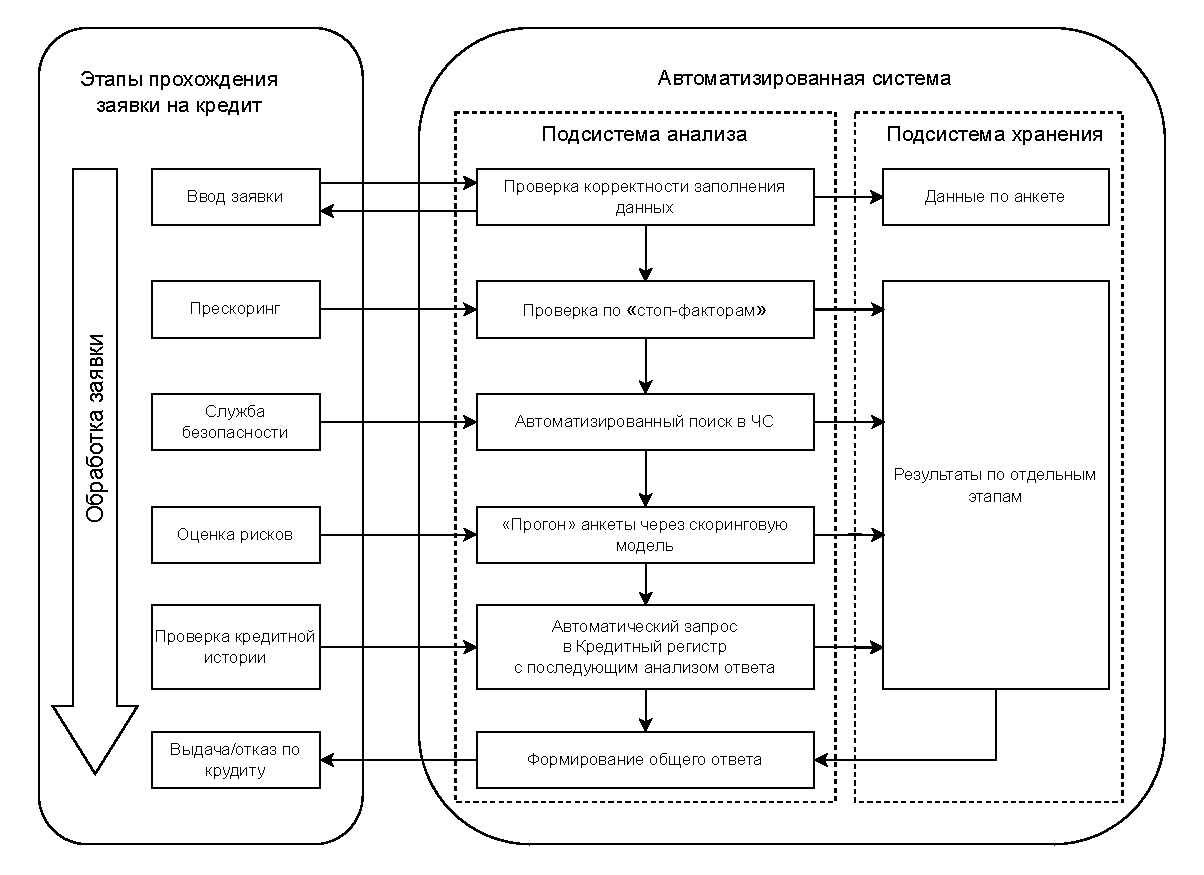
\includegraphics[width=\linewidth]{inc/pdf/Общая схема бизнес-процесса принятия кредитного решения.pdf}
  \end{center}
  \captionsetup{justification=centering}
  \caption{Общая схема бизнес-процесса принятия кредитного решения}
  \label{fig1::scoring schema}
\end{figure}
\FloatBarrier

\newpage
Скоринговые системы, особенно в условиях использования больших данных, должны соответствовать ряду требований, чтобы эффективно выполнять свои функции. Архитектура системы должна быть масштабируемой, чтобы увеличивать ее мощность по мере роста данных и требований. Также требуется возможность бесшовной интеграции с существующими банковскими системами, базами данных и IT-инфраструктурой, а также обеспечение защиты данных от несанкционированного доступа, утечек и кибератак.

Функциональные требования предусматривают применение скоринговых моделей для оценки кредитного риска с минимальной ошибкой.
Важным условием является способность системы быстро обновлять модели и алгоритмы в ответ на изменения рынка и поведения клиентов.

%\subsection{Обзор существующих методов}
%---------------------------------------------------
\subsection{Градиентный бустинг деревьев решений}

Градиентный бустинг -- это техника машинного обучения для задач классификации и регрессии, которая строит модель предсказания в
форме ансамбля слабых предсказывающих моделей. При этом обучение ансамбля проводится последовательно.

Градиентный бустинг с деревьями решений в качестве базовых моделей называется GBDT.
Он способен эффективно находить нелинейные зависимости в данных различной природы. Этим свойством обладают все алгоритмы, использующие деревья решений \cite{Kornienko}.

\textbf{Постановка задачи}

Рассмотрим задачу обучения с учителем, где имеется обучающая выборка из $n$ наблюдений:

\begin{equation}
  D = \{(x_i, y_i)\}_{i=1}^{n},
\end{equation}

где
\begin{itemize}
  \item $x_i \in \mathbb{R}^{d}$ --- вектор признаков;
  \item $y_i \in \mathbb{R}$ --- целевая переменная;
  \item $n$ --- количество наблюдений в обучающей выборке;
  \item $d$ --- количество признаков.
\end{itemize}

Цель состоит в построении модели $F(x)$, которая предсказывает значение $y$ для нового объекта $x$.

\textbf{Общая идея градиентного бустинга}

Градиентный бустинг строит модель в виде ансамбля базовых моделей:

\begin{equation}
  F(x) = F_0(x) + \sum_{m=1}^{M} \gamma_m h_m(x),
\end{equation}

где
\begin{itemize}
  \item $F_0(x)$ --- начальное приближение модели;
  \item $M$ --- количество базовых моделей;
  \item $m$ --- номер базовой модели;
  \item $\gamma_m$ --- коэффициент шага на $m$-й итерации;
  \item $h_m(x)$ --- базовая модель на $m$-й итерации.
\end{itemize}

\textbf{Выбор функции потерь}


Выбирается дифференцируемая функция потерь, которая измеряет расхождение между истинными значениями и предсказаниями модели. Для задачи классификации может использоваться логистическая функция потерь:

\begin{equation}
  L(y, F(x)) = \ln\left(1 + e^{-2yF(x)}\right), \quad y \in \{-1, +1\}.
\end{equation}


\textbf{Алгоритм градиентного бустинга}

Шаг 1. Устанавливается начальное приближение модели таким образом, чтобы минимизировать функцию потерь на обучающей выборке:
\begin{equation}
  F_0(x) = \arg\min_{\gamma} \sum_{i=1}^{n} L(y_i, \gamma),
\end{equation}

где

\begin{itemize}
  \item $\gamma$ --- постоянное значение, подбираемое при минимизации функции потерь;
  \item $i$ --- номер наблюдения в обучающей выборке.
\end{itemize}


Для логистической функции потерь начальное приближение может быть задано следующим образом:

\begin{equation}
  F_0(x) = \frac{1}{2} \ln\left(\frac{p}{1-p}\right), \quad p = \frac{1}{n} \sum_{i=1}^{n} y_i,
\end{equation}

где $p$ --- среднее значение целевой переменной в обучающей выборке.

Шаг 2. Для каждой итерации от $1$ до $M$ выполняются следующие действия.

а) Вычисляются псевдоостатки. Псевдоостатки определяются как отрицательный градиент функции потерь по предсказанию текущей модели:

\begin{equation}
  r_{im} = -\left[\frac{\partial L(y_i, F(x_i))}{\partial F(x_i)}\right]_{F(x) = F_{m-1}(x)},
\end{equation}

где $F_{m-1}(x)$ --- модель, полученная на предыдущей итерации.

б) Базовая модель обучается на данных, где псевдоостатки используются как целевая переменная:

\begin{equation}
  h_m(x) \approx r_{im}.
\end{equation}

в) Вычисляется коэффициент шага. Оптимальное значение коэффициента шага находится путем минимизации функции потерь:

\begin{equation}
  \gamma_m = \arg\min_{\gamma} \sum_{i=1}^{n} L\left(y_i, F_{m-1}(x_i) + \gamma h_m(x_i)\right).
\end{equation}

г) Обновляется текущее приближение модели:

\begin{equation}
  F_m(x) = F_{m-1}(x) + \gamma_m h_m(x).
\end{equation}

Шаг 3. После выполнения $M$ итераций получается итоговая модель:

\begin{equation}
  F_M(x) = F_0(x) + \sum_{m=1}^{M} \gamma_m h_m(x).
\end{equation}

Градиентный бустинг является гибким ансамблевым методом, в котором итоговая модель строится последовательно за счет добавления базовых алгоритмов, уменьшающих значение выбранной функции потерь. Такой подход позволяет применять бустинг как в задачах регрессии, так и в задачах классификации, поскольку алгоритм может быть адаптирован к различным дифференцируемым функциям потерь. Дополнительное использование малой скорости обучения и других приемов регуляризации позволяет повысить обобщающую способность модели и снизить риск переобучения \cite{HastieElementsBoosting}.

А также, модель остается интерпретируемой, так как вес каждого дерева и важность признаков можно анализировать для получения полезной информации \cite{Lebedev}.

Однако у алгоритма есть и свои недостатки. Одной из главных проблем является длительное время обучения, поскольку обучение каждого дерева выполняется последовательно, что замедляет работу на больших наборах данных. Кроме того, градиентный бустинг чувствителен к выбору гиперпараметров, таких как глубина деревьев или скорость обучения $(\gamma)$ что требует тщательной настройки. Еще одним недостатком является склонность к переобучению, если не использовать регуляризацию, например, ограничение глубины деревьев или мини-батчи. Наконец, модель плохо переносит значительные изменения в тренировочной выборке, так как в таких случаях ее приходится обучать с нуля.

Для практического применения градиентного бустинга на больших наборах данных используются оптимизированные реализации, такие как XGBoost и LightGBM. XGBoost представляет собой масштабируемую систему градиентного бустинга над деревьями решений, в которой применяются алгоритмы обработки разреженных данных, приближенного поиска разбиений, а также оптимизации доступа к памяти и распределенных вычислений \cite{ChenXGBoost}. LightGBM, в свою очередь, ориентирован на повышение скорости обучения и снижение потребления памяти за счет использования методов Gradient-based One-Side Sampling и Exclusive Feature Bundling, что делает данный алгоритм эффективным при работе с большими объемами данных \cite{KeLightGBM}.


%-------------------------------------------

\subsection{Логистическая регрессия}

Логистическая регрессия применяется в задачах, где зависимая переменная имеет бинарный характер и принимает одно из двух возможных значений. В отличие от обычной линейной регрессии, данный метод используется не для непосредственного прогнозирования числового значения признака, а для оценки вероятности наступления определенного события. В модели логистической регрессии вероятность события преобразуется через шансы и логиты, что позволяет представить связь между зависимой переменной и набором независимых признаков в виде линейной комбинации предикторов \cite{PampelLogisticRegression}.

В банковских скоринговых системах логистическая регрессия используется для оценки вероятности дефолта, ранжирования клиентов по риску или интерпретации влияния признаков на вероятность дефолта.

Логистическая регрессия моделирует вероятность события $y = 1$ в зависимости от вектора признаков $x$ с использованием логистической функции (сигмоиды):

\begin{equation}
  P(y = 1 \mid x) = \sigma(z) = \frac{1}{1 + e^{-z}},
\end{equation}

где

\begin{itemize}
  \item $z = w^T x + b$ --- линейная комбинация признаков;
  \item $w$ --- вектор весов модели;
  \item $b$ --- смещение.
\end{itemize}

Цель обучения логистической регрессии -- найти такие параметры $w$ и $b$ которые минимизируют функцию потерь и обеспечивают наилучшее соответствие между предсказанными вероятностями и фактическими метками классов.

\textbf{Математическое описание}

Для набора данных из $n$ наблюдений $\{(x_i, y_i)\}_{i=1}^{n}$ функция правдоподобия модели выражается следующим образом:

\begin{equation}
  L(w, b) = \prod_{i=1}^{n} P(y_i \mid x_i) =
  \prod_{i=1}^{n} \left[\sigma(w^T x_i + b)\right]^{y_i}
  \left[1 - \sigma(w^T x_i + b)\right]^{1 - y_i},
\end{equation}

где
\begin{itemize}
  \item $P(y_i \mid x_i)$ --- условная вероятность принадлежности объекта $x_i$ к классу $y_i$;
  \item $\sigma$ --- сигмоидная функция;
  \item $w$ --- вектор весов модели;
  \item $b$ --- смещение модели.
\end{itemize}

Для удобства оптимизации используется отрицательный логарифм функции правдоподобия, известный как логистическая функция потерь:

\begin{equation}
  J(w, b) = -\sum_{i=1}^{n} \left[
    y_i \ln \sigma(w^T x_i + b) +
    (1 - y_i) \ln \left(1 - \sigma(w^T x_i + b)\right)
    \right],
\end{equation}

где $J(w, b)$ --- логистическая функция потерь.

Параметры модели обновляются с помощью градиентного спуска путем минимизации функции потерь:

\begin{equation}
  w := w - \eta \frac{\partial J(w, b)}{\partial w}, \quad
  b := b - \eta \frac{\partial J(w, b)}{\partial b},
\end{equation}

где $\eta$ --- скорость обучения.

Для нового объекта $x$ оценивается вероятность $P(y = 1 \mid x)$. Если вероятность превышает заданный порог, объект классифицируется как положительный класс:

\begin{equation}
  \hat{y} =
  \begin{cases}
    1, & \text{если } P(y = 1 \mid x) \geqslant 0{,}5, \\
    0, & \text{иначе},
  \end{cases}
\end{equation}

где $\hat{y}$ --- предсказанная метка класса.

Ключевыми преимуществами логистической регрессии являются простота и интерпретируемость. Модель легко объяснима, что особенно важно для финансовых организаций и для соответствия нормативным требованиям. Кроме того, логистическая регрессия характеризуется эффективностью вычислений; обучение модели происходит относительно быстро, даже на больших наборах данных. Также при правильной регуляризации модель демонстрирует устойчивость к переобучению, будучи менее подверженной этому риску по сравнению с более сложными алгоритмами \cite{Marmish}.

Логистическая регрессия имеет и некоторые ограничения. Одно из них -- линейность модели, которая предполагает линейную зависимость между признаками и логарифмом шансов. Это может быть недостаточно для моделирования сложных нелинейных зависимостей. Модель также чувствительна к выбросам и масштабированию признаков, поэтому требуется предварительная обработка данных, включая нормализацию и обработку выбросов. Ограниченная выразительная способность логистической регрессии может привести к тому, что она будет уступать более сложным моделям, таким как градиентный бустинг, в точности предсказаний на сложных данных.

%--------------------------------------

\subsection{Линейный дискриминантный анализ}

Линейный дискриминантный анализ относится к методам многомерной классификации и применяется в случаях, когда классы объектов заранее известны. Основная задача метода заключается в построении дискриминантной функции, позволяющей отнести новый объект к одному из существующих классов на основании значений его признаков. В линейном случае такая функция задается как линейная комбинация исходных показателей, параметры выбираются так, чтобы обеспечить наилучшее разделение рассматриваемых групп \cite{OrlovaDiscriminantAnalysis}. Скоринговый балл рассчитывается как линейная функция от значений атрибутов клиента:

\begin{equation}
  Z = \beta^T x = \beta_1 x_1 + \beta_2 x_2 + \ldots + \beta_k x_k,
\end{equation}

где

\begin{itemize}
  \item $x = (x_1, \ldots, x_k)$ --- вектор значений атрибутов клиента;
  \item $x_1, x_2, \ldots, x_k$ --- отдельные атрибуты клиента;
  \item $\beta = (\beta_1, \ldots, \beta_k)$ --- вектор параметров модели;
  \item $\beta_1, \beta_2, \ldots, \beta_k$ --- параметры модели;
  \item $k$ --- количество атрибутов клиента.
\end{itemize}


\newpage
Параметры модели выбираются таким образом, чтобы максимизировать отношение:

\begin{equation}
  M = \frac{\beta^T (m_G - m_B)}{\sqrt{\beta^T \Sigma \beta}},
\end{equation}
где
\begin{itemize}
  \item $M$ --- значение критерия разделения классов;
  \item $m_G$ --- вектор средних значений признаков для хороших клиентов;
  \item $m_B$ --- вектор средних значений признаков для плохих клиентов;
  \item $\Sigma$ --- общая ковариационная матрица.
\end{itemize}

Недостатком является то, что ЛДА требует нормально распределенных данных, но данные о кредитных операциях часто являются слабоструктурированными и не всегда есть возможность их классифицировать.

Линейный дискриминантный анализ предполагает равенство ковариационных матриц
и нормальное распределение независимых переменных. В задачах кредитного
скоринга эти предположения часто нарушаются, поскольку признаки могут быть
дискретными или не подчиняться нормальному распределению. Это усложняет
применение метода. Однако показано, что при нарушении условия
данный метод остается применим на практике \cite{Petuhov}.

Схожий метод линейной регрессии, также используется для формирования скоринговой модели. В случае двух категорий, он эквивалентен методу линейного дискриминантного анализа и выражает зависимость одной переменный (зависимой) от других (независимых). В общем виде представляется так:

\begin{equation}
  Y = \beta_0 + \beta_1 X_1 + \ldots + \beta_n X_n + \epsilon,
\end{equation}

где

\begin{itemize}
  \item $Y$ --- зависимая переменная;
  \item $\beta_0$ --- свободный член модели;
  \item $X_i$ --- объясняющая независимая переменная;
  \item $\beta_i$ --- коэффициент регрессии при переменной $X_i$;
  \item $n$ --- количество объясняющих переменных;
  \item $\epsilon$ --- случайная ошибка.
\end{itemize}

Для применения модели линейного скоринга требуется выполнение следующего предположения: связь между зависимой и независимыми переменными должна быть линейной. В противном случае, точность оценки значительно ухудшается. Ошибки же должны быть независимы и распределены нормально.

Как и в случае дискриминантного анализа, в условиях кредитного скоринга, предположения, требуемые для применения линейной регрессии, нередко нарушаются. Линейная регрессия может дать оценку вероятности вне диапазона [0,1], что является неприемлемым.


\subsection{Метод опорных векторов}

Метод опорных векторов (support vector machine, SVM) относится к методам интеллектуального анализа данных для решения задачи классификации. Его основная идея заключается в переводе исходных векторов в пространство более высокой размерности c применением метода ядра для обеспечения линейной разделимости классов и в поиске разделяющей гиперплоскости с максимальным зазором между гиперплоскостью и опорными векторами в этом пространстве \cite{Mihailov}.

\textbf{Постановка задачи}

Пусть имеется обучающая выборка:
\begin{equation}
  D = \{(x_i, y_i)\}_{i=1}^{n}, \quad x_i \in \mathbb{R}^{d}, \quad y_i \in \{-1, +1\}.
\end{equation}

Метод SVM строит разделяющую гиперплоскость, минимизируя ошибку классификации и максимизируя зазор между классами:

\begin{equation}
  \mathcal{H}(w, b) = \{x \in \mathbb{R}^{d} : w^T x + b = 0\},
\end{equation}

где $w$ --- вектор нормали к гиперплоскости.
\newpage
\textbf{Оптимизационная задача SVM}

Для линейно разделимых данных SVM решает следующую задачу оптимизации:
\begin{equation}
  \min_{w, b} \frac{1}{2} \|w\|^2,
  \quad \text{при ограничениях } y_i (w^T x_i + b) \geqslant 1, \quad \forall i.
\end{equation}

Данная формулировка минимизирует норму вектора $w$, что эквивалентно максимизации зазора между классами.

Для линейно неразделимых данных вводится штраф за ошибочную классификацию с использованием мягкого зазора:

\begin{equation}
  \min_{\mathbf{w}, b, \xi} \frac{1}{2} \|\mathbf{w}\|^2 + C \sum_{i=1}^{n} \xi_i,
  \quad \text{при ограничениях } y_i (\mathbf{w}^T \mathbf{x}_i + b) \geqslant 1 - \xi_i,
  \quad \xi_i \geqslant 0, \quad \forall i,
\end{equation}

где $C$ --- гиперпараметр, регулирующий допустимый уровень ошибок при построении разделяющей гиперплоскости.


На рисунке \ref{fig2:SVM schema} показана разница между идеальным разделением классов (hard margin) и случаем с допущением ошибок классификации (soft margin). В случае мягкого зазора некоторые точки могут находиться внутри разделяющей полосы или за ее пределами, что учитывается через переменные \(\xi_i\).

\begin{figure}[ht]
  \begin{center}
    {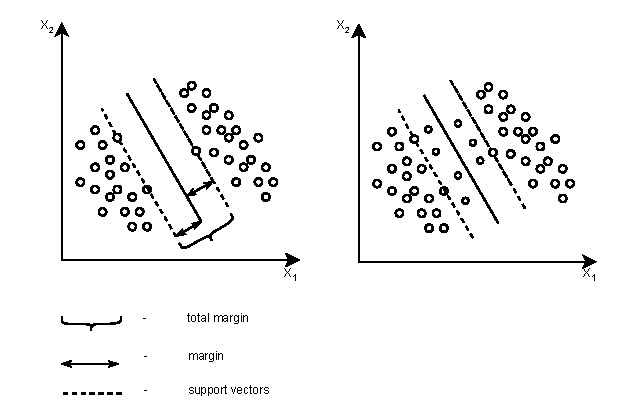
\includegraphics[scale = 0.8]{inc/pdf/Принцип работы линейного SVM с жёстким и мягким зазором.pdf}}
    \caption{Принцип работы линейного SVM с жестким и мягким зазором}
    \label{fig2:SVM schema}
  \end{center}
\end{figure}

\textbf{Ядерный метод в SVM}

Для линейно неразделимых данных в исходном пространстве SVM использует ядра, которые позволяют перенести данные в пространство более высокой размерности, где классы становятся линейно разделимыми. Скалярное произведение в новом пространстве, неявно заданном отображением $\phi(x)$, вычисляется с помощью ядерной функции $K(x_i, x_j)$:

\begin{equation}
  K(x_i, x_j) = \gamma(x_i)^T \gamma(x_j).
\end{equation}

\textbf{Решение двойственной задачи}

SVM решает двойственную задачу оптимизации, что позволяет использовать ядра:

\begin{equation}
  \max_{\alpha} \sum_{i=1}^{n} \alpha_i
  - \frac{1}{2} \sum_{i=1}^{n} \sum_{j=1}^{n}
  \alpha_i \alpha_j y_i y_j K(x_i, x_j),
\end{equation}

где

\begin{itemize}
  \item $\alpha_i$ --- коэффициент, определяющий важность $i$-го объекта;
  \item $j$ --- номер объекта в обучающей выборке;
  \item $K(x_i, x_j)$ --- ядерная функция, определяющая меру сходства объектов $x_i$ и $x_j$.
\end{itemize}

При этом выполняются следующие ограничения:

\begin{equation}
  0 \leq \alpha_i \leq C, \quad \sum_{i=1}^{n} \alpha_i y_i = 0.
\end{equation}

Только объекты, лежащие на границах зазора или внутри него, то есть опорные векторы, имеют ненулевые значения $\alpha_i$ и влияют на итоговую модель.

Метод опорных векторов (SVM) находит широкое применение в кредитном скоринге, где требуется оценить вероятность выполнения клиентом определенных обязательств. SVM решает задачу бинарной классификации, разделяя клиентов на платежеспособных и неплатежеспособных.

Скоринг формулируется как задача бинарной классификации: положительный класс ($y = +1$) соответствует платежеспособным клиентам, а отрицательный класс ($y = -1$) -- неплатежеспособным. Входные признаки $x_i$ включают данные о клиенте, такие как возраст, доход, кредитная история и другие характеристики. На основе обучающей выборки, содержащей исторические данные о клиентах, SVM строит оптимальную разделяющую гиперплоскость. Для повышения качества модели может использоваться мягкий зазор (soft margin), позволяющий учитывать ошибки классификации. Полученный результат классификации преобразуется в числовой балл, отражающий уровень риска клиента:

\begin{equation}
  \text{Score} = w^T x + b,
\end{equation}

где

\begin{itemize}
  \item $\text{Score}$ --- скоринговый балл, отражающий уровень риска клиента;
  \item $x$ --- вектор признаков клиента;
  \item $b$ --- смещение модели.
\end{itemize}

Положительное значение $\text{Score}$ указывает на низкий риск дефолта, а отрицательное --- на высокий.

Преимуществами метода опорных векторов (SVM) являются высокая скорость нахождения решающих функций и возможность свести задачу к решению квадратичного программирования в выпуклой области, которая всегда имеет единственное решение. Кроме того, SVM находит разделяющую гиперплоскость с максимальной шириной полосы, что позволяет осуществлять более уверенную классификацию.

Однако метод чувствителен к шумам и требует тщательной стандартизации данных. Отсутствует общий подход к выбору ядра и построению спрямляющего подпространства при работе с линейно неразделимыми классами. SVM также плохо масштабируется на большие объемы данных, так как решает задачу квадратичного программирования, сложность которой растет квадратично или кубически с увеличением размера обучающей выборки. Шумы в данных могут оказывать существенное влияние на положение разделяющей гиперплоскости, особенно при использовании мягкого зазора, так как ошибочно классифицированные объекты могут стать опорными векторами. Метод требует тщательной предварительной обработки данных, включая нормализацию или стандартизацию признаков и управление выбросами, чтобы минимизировать влияние масштаба данных и выбросов на результат модели \cite{Xiangdong}.


\subsection{Классификация существующих решений}

В качестве основных параметров классификации алгоритмов были использованы признаки, приведенные в таблице \ref{tab:type_classification}:

\begin{table}[ht]
  \centering
  \caption{Параметры классификации алгоритмов}
  \label{tab:type_classification}
  \begin{tabular}{|c|p{0.9\textwidth}|}
    \hline
    \textbf{} & \textbf{Параметр}                                                                            \\
    \hline
    1         & Способность модели прогнозировать целевую переменную (например, вероятность дефолта клиента) \\
    2         & Тип модели                                                                                   \\
    3         & Параметричность                                                                              \\
    4         & Масштабируемость и обработка больших данных                                                  \\
    5         & Предположения о данных                                                                       \\
    6         & Устойчивость к переобучению и шуму                                                           \\
    7         & Тип алгоритма                                                                                \\
    8         & Способность моделировать сложные зависимости                                                 \\
    9         & Требования к предварительной обработке данных                                                \\
    10        & Устойчивость к выбросам                                                                      \\
    11        & Время обучения и предсказания                                                                \\
    12        & Совместимость с технологиями больших данных                                                  \\
    13        & Поддержка параллельных вычислений и распределенной обработки данных                          \\
    \hline
  \end{tabular}
\end{table}

\newpage
Классификация существующих алгоритмов представлена в таблице \ref{tab:method_classification}.

{\footnotesize   % уменьшение шрифта
\sloppy % более либеральный подход к разрыву строк
\hyphenpenalty=10000 % запрет переносов слов по слогам
\exhyphenpenalty=10000 % запрет переносов при наличии дефисов

\begin{longtable}{|p{3cm}|p{3cm}|p{3cm}|p{3cm}|p{3cm}|}
  \caption{Таблица сравнения существующих алгоритмов} \label{tab:method_classification}                                                                                                                                                                                                                                                                                                          \\
  \hline
  \textbf{Критерий}                                                            & \textbf{Градиентный бустинг деревьев решений}                                       & \textbf{Логистическая регрессия}                      & \textbf{Линейный дискриминантный анализ}                                      & \textbf{Метод опорных векторов (SVM)}                                             \\ \hline
  \endfirsthead

  % ИСПРАВЛЕНО: l -> c для центрирования
  \multicolumn{5}{c}{\normalsize Продолжение таблицы \ref{tab:method_classification}}                                                                                                                                                                                                                                                                                                            \\ \hline
  \textbf{Критерий}                                                            & \textbf{Градиентный бустинг деревьев решений}                                       & \textbf{Логистическая регрессия}                      & \textbf{Линейный дискриминантный анализ}                                      & \textbf{Метод опорных векторов (SVM)}                                             \\ \hline
  \endhead

  \endfoot

  \hline
  \endlastfoot

  \textbf{Способность модели точно прогнозировать целевую переменную}          & Высокая точность за счет сложных нелинейных зависимостей                            & Умеренная точность при линейных зависимостях          & Точность зависит от выполнения предположений о данных                         & Высокая, при правильном выборе ядра                                               \\ \hline
  \textbf{Тип модели}                                                          & Нелинейная                                                                          & Линейная                                              & Линейная                                                                      & Нелинейная                                                                        \\ \hline
  \textbf{Параметричность}                                                     & Непараметрическая                                                                   & Параметрическая                                       & Параметрическая                                                               & Непараметрическая                                                                 \\ \hline
  \textbf{Обработка больших данных}                                            & Высокая (с библиотеками)                                                            & Высокая                                               & Средняя                                                                       & Низкая; плохо масштабируется на большие выборки                                   \\ \hline
  \textbf{Предположения о данных}                                              & Минимальные                                                                         & Линейность, независимость признаков                   & Нормальность, равенство ковариаций                                            & Минимальные, но требуется стандартизация данных                                   \\ \hline
  \textbf{Устойчивость к переобучению и шуму}                                  & Требует настройки гиперпараметров для предотвращения переобучения                   & Устойчива при использовании регуляризации             & Чувствительна к выбросам и нарушениям предположений                           & Чувствителен к шумам, но настраиваемый параметр \(C\) помогает снизить их влияние \\ \hline
  \textbf{Тип алгоритма}                                                       & Ансамблевый метод (бустинг)                                                         & Одиночная модель                                      & Одиночная модель                                                              & Одиночная модель                                                                  \\ \hline
  \textbf{Способность моделировать сложные зависимости}                        & Высокая                                                                             & Ограничена (только линейные зависимости)              & Ограничена линейностью модели                                                 & Высокая, при использовании нелинейных ядер                                        \\ \hline
  \textbf{Требования к предварительной обработке данных}                       & Низкие; не требует масштабирования признаков                                        & Высокие; требует масштабирования и обработки выбросов & Высокие; требует нормальности распределения и равенства ковариационных матриц & Высокие; требует масштабирования и удаления выбросов                              \\ \hline
  \textbf{Устойчивость к выбросам}                                             & Относительно устойчива                                                              & Чувствительна к выбросам                              & Очень чувствительна к выбросам                                                & Чувствителен к выбросам                                                           \\ \hline
  \textbf{Время обучения и предсказания}                                       & Длительное обучение; быстрое предсказание                                           & Быстрое обучение и предсказание                       & Обучение может быть медленным из-за вычисления ковариационных матриц          & Медленное обучение; быстрое предсказание                                          \\ \hline
  \textbf{Совместимость с технологиями больших данных}                         & Да; поддерживается оптимизированными библиотеками (XGBoost, LightGBM)               & Да; легко интегрируется                               & Ограничена; требует дополнительных усилий для интеграции                      & Ограничена; требует модификаций для больших данных                                \\ \hline
  \textbf{Поддержка параллельных вычислений и распределенной обработки данных} & Да; оптимизированные библиотеки используют многоядерные и распределенные вычисления & Ограничена; в базовой реализации требуется настройка  & Ограничена; требует существенных усилий для распараллеливания                 & Ограничена; базовые реализации не поддерживают распараллеливание                  \\ \hline
\end{longtable}
}


%\subsection{Обзор существующих систем кредитного скоринга}

\subsection{Скоринговая система FICO}

FICO Score является одной из наиболее распространенных скоринговых систем, используемых кредиторами для оценки кредитного риска заемщиков. Данный показатель рассчитывается на основе информации, содержащейся в кредитной истории клиента, и обычно находится в диапазоне от 300 до 850 баллов. Более высокое значение FICO Score соответствует более низкому уровню риска для кредитора и может положительно влиять на вероятность одобрения кредита и условия его предоставления \cite{MyFicoCreditScores}.

Расчет FICO Score основывается на анализе кредитной истории заемщика и включает несколько ключевых факторов:

\begin{itemize}
  \item платежная дисциплина (около 35\%) -- своевременность погашения задолженностей;
  \item уровень задолженности (около 30\%) -- отношение текущих обязательств к доступному кредитному лимиту;
  \item длительность кредитной истории (около 15\%);
  \item структура кредитов (около 10\%) -- разнообразие кредитных продуктов;
  \item новые кредитные заявки (около 10\%).
\end{itemize}

Модель FICO относится к классу проприетарных решений, что означает отсутствие открытой информации о точных алгоритмах расчета. Однако известно, что в основе системы лежат статистические методы анализа данных, включая элементы логистической регрессии и скоринговых карт.

К преимуществам системы FICO можно отнести широкое распространение, стандартизацию оценки кредитного риска и высокую интерпретируемость результатов. Вместе с тем, использование фиксированной модели ограничивает ее адаптивность к изменениям в поведении заемщиков и особенностям локальных рынков.

Система FICO представляет собой классический пример промышленного скорингового решения, на основе которого развиваются современные методы оценки кредитоспособности, включая модели машинного обучения.

\subsection{Скоринговые решения Experian}

Решения Experian в области кредитного скоринга и принятия решений ориентированы на автоматизацию кредитного процесса и управление рисками на различных этапах жизненного цикла клиента. В качестве одного из таких решений используется платформа PowerCurve, предназначенная для объединения данных, аналитики и технологий принятия решений в единой системе. Данная платформа позволяет автоматизировать кредитные решения, использовать аналитические модели и учитывать информацию, связанную с кредитным риском, проверкой клиента и противодействием мошенничеству.

Современные решения Experian используют не только традиционные данные кредитной истории, но и расширенные источники информации, а также методы аналитики и машинного обучения. Это позволяет преобразовывать сложные данные в прикладные решения для оценки риска, управления портфелем, привлечения клиентов и сопровождения кредитного процесса.

К основным возможностям решений Experian относятся:

\begin{itemize}
  \item построение и настройка скоринговых моделей под конкретные бизнес-задачи;
  \item использование как традиционных, так и альтернативных источников данных;
  \item интеграция с внутренними банковскими системами и внешними сервисами;
  \item автоматизация процесса принятия решений в кредитном конвейере;
  \item мониторинг и управление кредитным риском в режиме реального времени;
  \item применение методов машинного обучения для повышения качества прогнозирования.
\end{itemize}

Преимуществом решений Experian является их высокая адаптивность и возможность учитывать изменения в поведении клиентов и рыночной среде. Использование больших данных и методов машинного обучения позволяет существенно повысить точность скоринговых моделей по сравнению с традиционными подходами.

Внедрение подобных систем связано с рядом сложностей, включая необходимость обработки больших объемов данных, обеспечение их качества, а также наличие вычислительных ресурсов и квалифицированных специалистов.

Таким образом, решения Experian представляют собой современные скоринговые системы, использующие методы анализа больших данных и машинного обучения, что делает их более гибкими и эффективными по сравнению с классическими скоринговыми моделями.

\subsection{Скоринговые системы на основе машинного обучения}

Современное развитие кредитного скоринга связано с активным применением методов машинного обучения для автоматизированной оценки кредитных рисков. Такие методы позволяют анализировать большие объемы клиентских данных, выявлять сложные зависимости между признаками заемщика и вероятностью дефолта, а также повышать качество прогнозирования по сравнению с рядом традиционных статистических подходов.

В задачах оценки кредитного риска применяются различные алгоритмы машинного обучения, включая логистическую регрессию, метод k-ближайших соседей, деревья решений, случайный лес и градиентный бустинг. Особое значение имеют ансамблевые методы, так как они позволяют объединять несколько моделей и повышать устойчивость итогового прогноза \cite{ChubCreditRiskML}.

Наиболее распространенными инструментами для построения таких моделей являются библиотеки и платформы анализа данных, такие как:

\begin{itemize}
  \item Scikit-learn -- библиотека машинного обучения на языке Python;
  \item XGBoost -- высокоэффективная реализация градиентного бустинга;
  \item LightGBM -- оптимизированный алгоритм бустинга для работы с большими данными;
  \item CatBoost -- алгоритм градиентного бустинга, эффективно работающий с категориальными признаками.
\end{itemize}

Использование методов машинного обучения позволяет учитывать сложные нелинейные зависимости между признаками, а также эффективно работать с большими объемами данных. Это приводит к повышению точности оценки кредитного риска по сравнению с традиционными подходами.

Вместе с тем, такие модели обладают меньшей интерпретируемостью, что может затруднять их использование в условиях строгого регулирования финансового сектора. В связи с этим на практике часто применяются гибридные подходы, сочетающие интерпретируемые модели и алгоритмы машинного обучения.

Таким образом, использование методов машинного обучения является современным направлением развития скоринговых систем и представляет собой перспективную основу для построения моделей оценки кредитоспособности.



\subsection{Формулировка цели}

В ходе выполнения работы требуется разработать модель, позволяющая оценивать кредитоспособность физических лиц в банковских системах с использованием алгоритма градиентного бустинга деревьев решений. Разрабатываемая модель должна отвечать следующим требованиям:

\begin{enumerate}
  \item Обеспечивать высокую точность прогнозирования вероятности дефолта заемщика.
  \item Учитывать совокупность финансовых и социально-демографических характеристик клиента.
  \item Обеспечивать возможность работы с большими объемами данных.
  \item Обладать устойчивостью к шумам и выбросам в данных.
  \item Обеспечивать приемлемое время обучения и предсказания.
  \item Позволять интерпретировать результаты оценки кредитного риска.
\end{enumerate}

\subsection{Формализация задачи. IDEF0-диаграмма}
Для формализации задачи была составлена IDEF0-диаграмма нулевого и первого уровня.

IDEF0-диаграмма нулевого уровня представлена на рисунке \ref{idef0::0}:

\FloatBarrier
\begin{figure}[ht]
  \begin{center}
    
\includegraphics[height=8cm]{inc/png/01_A-0.png}
  \end{center}
  \captionsetup{justification=centering}
  \caption{IDEF0-диаграмма нулевого уровня}
  \label{idef0::0}
\end{figure}
\FloatBarrier

IDEF0-диаграмма нулевого уровня (A-0) отражает общий процесс оценки кредитоспособности заемщика.
На вход системы поступают анкетные данные клиента, финансовые данные и кредитная история.
Управляющими воздействиями выступают требования к методу, порог принятия решения и правила скоринговой модели.
В качестве механизмов используются алгоритм GBDT (ML модель) и программный комплекс оценки кредитоспособности.
Результатом выполнения процесса являются скоринговый балл, оценка кредитного риска и решение о выдаче кредита.

IDEF0-диаграмма первого уровня представлена на рисунке \ref{idef0::1}:

\FloatBarrier
\begin{figure}[ht]
  \begin{center}
    
\includegraphics[height=8cm]{inc/png/02_A0.png}
  \end{center}
  \captionsetup{justification=centering}
  \caption{IDEF0-диаграмма первого уровня}
  \label{idef0::1}
\end{figure}
\FloatBarrier

IDEF0-диаграмма первого уровня (A0) детализирует процесс оценки кредитоспособности заемщика и разбивает его на последовательные этапы.

На этапе A1 выполняется сбор и подготовка данных. На вход данного этапа поступают анкетные данные клиента, финансовые данные и кредитная история. Результатом этапа являются подготовленные данные.

На этапе A2 осуществляется предобработка данных. Подготовленные данные проходят обработку и преобразуются в обработанные данные, пригодные для дальнейшего расчета.

На этапе A3 выполняется расчет скорингового балла (GBDT) с использованием алгоритма GBDT (ML модель) и программного комплекса оценки кредитоспособности. На данный этап также воздействуют правила скоринговой модели. Результатом этапа является скоринговый балл.

На этапе A4 выполняется принятие решения по кредиту. На основе скорингового балла, порога принятия решения и требований к методу формируются итоговые результаты: решение о выдаче кредита, оценка кредитного риска и рекомендации.

Таким образом, декомпозиция позволяет выделить основные этапы обработки данных, расчета скорингового балла и принятия кредитного решения, а также показать взаимосвязь входных данных, управляющих воздействий, механизмов и результатов.

\subsection*{Выводы}

Был проведен анализ предметной области оценки кредитоспособности физических лиц, введены основные понятия кредитного скоринга. Рассмотрены методы машинного обучения, применяемые для оценки кредитного риска заемщиков, включая алгоритм градиентного бустинга деревьев решений.

Проанализированы традиционные статистические методы, такие как логистическая регрессия и линейный дискриминантный анализ, а также современные алгоритмы машинного обучения, включая метод опорных векторов и градиентный бустинг. Результаты сравнительного анализа представлены в табличном виде.

Была сформулирована цель работы. Постановка задачи формализована в виде IDEF0-диаграммы.